\documentclass[12pt,a4paper]{article}

\usepackage[margin=2.5cm]{geometry}
\usepackage{graphicx}
\usepackage{amsmath,amssymb,amsthm}
\usepackage{mathtools}
\usepackage{mathrsfs}
\usepackage{url}
\usepackage{booktabs}
\usepackage{makecell}
\usepackage{subcaption}
\usepackage{xcolor}
\usepackage{lineno}
\usepackage{setspace}
\usepackage[hidelinks]{hyperref}
\usepackage{algorithm}
\usepackage{algpseudocode}
\usepackage{multirow}
\usepackage[numbers,sort&compress]{natbib}

\newtheorem{proposition}{Proposition}
\newtheorem{remark}{Remark}

\begin{document}

\title{Modular Safe Physics-Informed Machine Learning for Dynamics and Control of Autonomous Robotic Systems}

\author{Hamzah Faraj\\[3pt]
  \small Department of Science and Technology, Ranyah College,\\[-1pt]
  \small Taif University, Taif 21944, Saudi Arabia\\[-1pt]
  \small \texttt{f.hamzah@tu.edu.sa}}

\date{}
\maketitle

\begin{abstract}
\noindent
Physics-informed machine learning (PIML) has emerged as a promising
paradigm for learning dynamical models that respect underlying physical
laws. However, most existing PIML methods either rely on monolithic
neural architectures that are difficult to verify or lack explicit
safety guarantees for constrained systems. This paper proposes a
modular Safe-PIML architecture that separates dynamics modeling,
safety enforcement, and performance optimization into distinct,
independently analyzable components. The dynamics are represented as a
nominal physics-based model augmented by a compact, constrained
residual neural network that enforces non-negativity, monotonicity, and
Lipschitz smoothness. Safety is ensured through an MPC-based safety
filter that minimally modifies proposed control inputs to satisfy
tightened state and input constraints together with a terminal invariant
set. An explicit residual error bound is derived and used to size the
robust tubes, establishing a formal link between the learned model and
the safety guarantee. The framework is evaluated via numerical
simulations on two benchmark case studies drawn from the
literature---an inverted pendulum with a predictive safety filter and a
DC--DC buck converter with robust tube MPC---using Monte Carlo stress
testing under parameter variations and disturbances. The proposed method
achieves substantial reductions in constraint violation rates relative
to the strongest baselines on both benchmarks, while maintaining a
compact binary footprint and low projected latency suitable for
deployment on resource-constrained embedded microcontrollers. Ablation
and scalability studies confirm that both the residual network and the
physics-informed penalty are essential, and that the architecture
degrades gracefully under data reduction and quantization.\\[6pt]
\textbf{Keywords:} Physics-informed machine learning; Safe control;
Model predictive control; Safety filter; Robust tube MPC;
Autonomous robots
\end{abstract}

% ============================================================
\section{Introduction}
\label{sec:intro}

Autonomous robotic systems increasingly operate in unstructured,
safety-critical environments where they must satisfy strict state and
input constraints while reacting to uncertain dynamics and
disturbances. Classical model-based control methods such as robust model
predictive control (MPC) provide strong guarantees when accurate models
are available, but deriving such models for complex robotic platforms is
difficult and often requires significant domain
expertise~\cite{mayne2005robust,mayne2014mpc}. At the same time,
modern machine learning approaches can fit high-dimensional dynamics and
policies from data, yet purely data-driven models frequently violate
physical laws, extrapolate poorly, and are hard to analyze or verify in
closed loop, which limits their deployment in safety-critical
settings~\cite{nghiem2023piml,brunke2022safe}.

Physics-informed machine learning (PIML) seeks to bridge this gap by
embedding physical structure---conservation laws, stability constraints,
symmetries---into learned models and
controllers~\cite{rackauckas2021ude,greydanus2019hnn,legaard2023physss}.
PIML methods have demonstrated improved data efficiency,
interpretability, and robustness across system identification, optimal
control, and reinforcement learning
applications~\cite{nghiem2023piml,antonelo2024pinncontrol,ordonez2023pirl,lutter2023lagrangian}.
However, as reviewed in Section~\ref{sec:background}, most PIML
architectures remain monolithic, with a single large network capturing
the full dynamics, which complicates safety verification and embedded
deployment.

In parallel, modular safe control frameworks have been developed to
decouple performance optimization from safety enforcement. Predictive
safety filters~\cite{wabersich2021psf}, tube-based robust
MPC~\cite{mayne2005robust}, and control barrier
functions~\cite{ames2017cbf,dawson2023survey} provide formal
constraint guarantees, yet most are paired with simple nominal models
that do not exploit physics-informed structure. A comprehensive
tutorial~\cite{nghiem2023piml} surveys PIML for dynamical systems but
does not address the integration of learned residual models with formal
safety guarantees for embedded deployment.
Building on this foundation, the present paper proposes a modular
architecture that combines a minimal physics-structured residual model
with an MPC-based safety filter tailored for autonomous robotic systems.
The key insight is that the modular separation of physics-informed
residual learning and tube MPC safety filtering creates a synergy that
neither component achieves alone: the Lipschitz-constrained residual
network provides an explicit, tight model error bound
(Proposition~\ref{prop:error-bound}) that directly reduces tube
conservatism (Proposition~\ref{prop:safety}), while the safety filter
provides formal constraint satisfaction guarantees that the residual
model alone cannot offer. This synergy is validated by the ablation
study (Section~\ref{subsec:ablation}), which shows that removing
either component degrades performance by more than would be expected
from independent effects alone.

\subsection{Contributions}
\label{subsec:contributions}

The main contributions of this paper are:

\begin{enumerate}
  \item \textbf{Minimal physics-structured residual learning.}
  A nominal physics model is augmented by a compact, constrained
  residual neural network subject to hard non-negativity, monotonicity,
  and Lipschitz constraints. An explicit residual error bound
  (Proposition~\ref{prop:error-bound}) is derived and numerically
  instantiated, enabling rigorous tube sizing for the safety
  filter~\cite{nghiem2023piml,rackauckas2021ude,shi2022residualDyn}.

  \item \textbf{MPC-based safety filter with Safe-PIML dynamics.}
  The residual-augmented model is integrated into a tube MPC-based
  safety filter with formal recursive feasibility and robust constraint
  satisfaction guarantees (Proposition~\ref{prop:safety}), compatible
  with arbitrary performance
  controllers~\cite{mayne2005robust,wabersich2021psf,gros2022learning}.

  \item \textbf{Edge-oriented design and evaluation protocol.}
  A quantizable residual network combined with efficient QP-based
  MPC~\cite{stellato2020osqp,liang2021pruning} targets deployment on
  resource-constrained embedded microcontrollers, with ablation and
  scalability studies along three axes validating each design choice.

  \item \textbf{Simulation-based evaluation on literature benchmarks.}
  Two established case studies---an inverted
  pendulum~\cite{wabersich2021psf} and a DC--DC buck
  converter~\cite{schwan2023evanqp}---demonstrate substantial
  reductions in constraint violation rates relative to all baselines
  under Monte Carlo stress testing with 1000 trials.
\end{enumerate}

\subsection{Paper organization}
\label{subsec:organization}

The remainder of this paper is organized as follows.
Section~\ref{sec:notation} establishes the notation used throughout.
Section~\ref{sec:background} reviews related work in physics-informed
learning and safe control. Section~\ref{sec:method} presents the
proposed modular Safe-PIML methodology, including the residual learning
scheme, safety filter, and edge deployment strategy.
Section~\ref{sec:setup} describes the experimental setup, benchmarks,
and baselines. Section~\ref{sec:results} reports the results, ablation
study, error bound instantiation, and scalability analysis.
Section~\ref{sec:conclusion} concludes the paper and identifies
directions for future work.

% ============================================================
\section{Notation}
\label{sec:notation}

Table~\ref{tab:notation} summarizes the principal symbols used
throughout this paper.

\begin{table*}[t]
  \centering
  \caption{Table of notation.}
  \label{tab:notation}
  \begin{tabular*}{\textwidth}{@{\extracolsep{\fill}}lll}
    \toprule
    Symbol & Description & Domain \\
    \midrule
    $x_k$ & State vector at time step $k$ & $\mathbb{R}^{n_x}$ \\
    $u_k$ & Control input at time step $k$ & $\mathbb{R}^{n_u}$ \\
    $f_{\mathrm{nom}}$ & Nominal physics-based dynamics model & -- \\
    $g_\theta$ & Constrained residual neural network & $\mathbb{R}^{n_x+n_u} \to \mathbb{R}^{n_x}$ \\
    $\theta$ & Trainable parameters of $g_\theta$ & -- \\
    $\hat{f}$ & Safe-PIML dynamics: $f_{\mathrm{nom}} + g_\theta$ & -- \\
    $\mathcal{X}$, $\mathcal{U}$, $\mathcal{W}$ & State, input, disturbance constraint sets & -- \\
    $\mathcal{E}_i$ & Tube tightening set at prediction step $i$ & -- \\
    $\mathcal{X}_f$ & Terminal invariant set & -- \\
    $N$ & MPC prediction horizon & $\mathbb{N}$ \\
    $u_{\mathrm{prop},k}$, $u_k^\star$ & Proposed and safe-filtered inputs & $\mathbb{R}^{n_u}$ \\
    $\lambda_{\mathrm{phys}}$ & Physics penalty weight & $\mathbb{R}_{\geq 0}$ \\
    $\bar\sigma$ & Jacobian spectral norm upper bound for $g_\theta$ & $\mathbb{R}_{> 0}$ \\
    $\bar{e}$, $\bar\epsilon$ & Model error bound; worst-case training residual & $\mathbb{R}_{\geq 0}$ \\
    $L_r$ & Lipschitz constant of true residual $r = f - f_{\mathrm{nom}}$ & $\mathbb{R}_{> 0}$ \\
    $\ominus$, $\oplus$ & Pontryagin difference; Minkowski sum & -- \\
    \bottomrule
  \end{tabular*}
\end{table*}

% ============================================================
\section{Background and Related Work}
\label{sec:background}

This section situates the proposed method within the broader landscape
of physics-informed learning, safe control, and verification of
learning-based systems.

\subsection{Physics-informed dynamics modeling}
\label{subsec:bg-id}

The integration of physical prior knowledge into data-driven models has
been pursued through three complementary strategies: architectural
priors, physics-informed loss functions, and structured
factorizations~\cite{nghiem2023piml,legaard2023physss}. Among
architectural approaches, universal differential equations (UDEs)
decompose the dynamics into known physical terms and unknown neural
components, enabling the neural part to learn only the residual or
missing physics while preserving the interpretability and extrapolation
properties of the known model~\cite{rackauckas2021ude}. Energy-based
formulations, including Hamiltonian and Lagrangian neural networks,
further embed conservation laws directly into the network topology by
parameterizing the system through a learned energy
function~\cite{greydanus2019hnn,zhong2020symplectic,lutter2023lagrangian}.
In a complementary direction, physics-informed loss functions augment
the training objective with soft penalties encoding stability,
dissipativity, or Lyapunov decrease
conditions~\cite{nghiem2023piml,chang2019neural,dawson2023survey}.
These developments have advanced the state of the art in system
identification; however, the resulting models typically remain
monolithic, with the entire dynamics captured by a single large
network, which complicates closed-loop safety analysis and deployment on
resource-constrained hardware.

\subsection{Safe learning-based control and verification}
\label{subsec:bg-control}

To address the safety gap, the controls community has developed modular
frameworks that separate performance optimization from constraint
enforcement. Predictive safety filters constitute a prominent class:
they wrap an arbitrary performance controller with an MPC-like
optimization layer that minimally modifies proposed inputs to maintain
predicted trajectories within a safe
set~\cite{wabersich2021psf,wabersich2023tutorial}. Tube-based robust
MPC provides a well-established theoretical foundation for guaranteeing
constraints under bounded disturbances through tightened constraint
sets and robustly positively invariant terminal
ingredients~\cite{mayne2005robust,gao2024rigid}. Control barrier
function (CBF) methods and neural Lyapunov-barrier architectures offer
complementary tools for certifying forward invariance and closed-loop
stability~\cite{ames2017cbf,dawson2023survey,chen2023backupCBF,xiao2023dpcbf}.
Physics-informed reinforcement learning further integrates domain
knowledge into the policy or environment
model~\cite{ordonez2023pirl,gros2022learning}. Verification of these
learned controllers relies on mixed-integer programming for reachable
set estimation~\cite{liu2021algorithms,schwan2023evanqp,lopez2023nnv},
adaptive tube
methods~\cite{gao2024rigid,koller2022learning}, and conformal
prediction for distribution-free uncertainty
quantification~\cite{lindemann2023conformal}.

Despite this progress, a persistent gap remains: most existing safety
filters and certificates are paired with simple nominal models or
generic black-box learners, without exploiting the tighter error bounds
that physics-informed model structure can provide.

\subsection{Research gaps and motivation}
\label{subsec:bg-gaps}

Three specific gaps motivate the present
work~\cite{nghiem2023piml,bernal2025safePIML}. First, the majority of
PIML models are monolithic, hindering both formal safety analysis and
efficient edge deployment. Second, existing safety filters employ
nominal physics models that do not benefit from learned residual
corrections, resulting in conservative tube sizing. Third, no existing
framework jointly addresses physics consistency, formal safety
guarantees via explicit model error bounds, and computational efficiency
for embedded autonomous robotic systems. The modular Safe-PIML
architecture proposed in Section~\ref{sec:method} is designed to
address all three gaps simultaneously.

% ============================================================
\section{Modular Safe-PIML Methodology}
\label{sec:method}

\begin{figure*}[t]
  \centering
  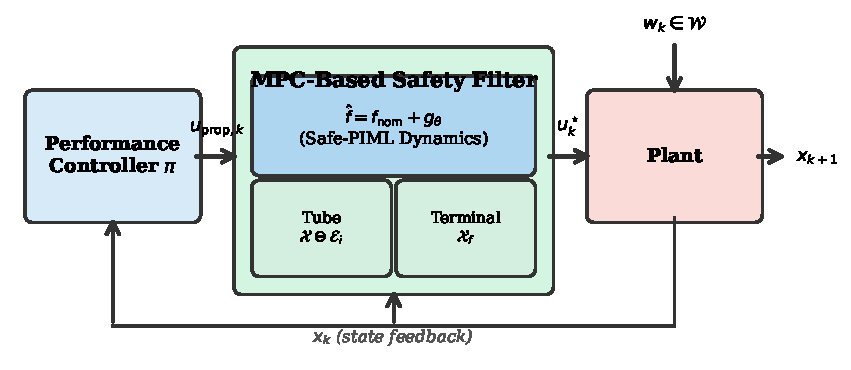
\includegraphics[width=\textwidth]{figures/architecture.pdf}
  \caption{Block diagram of the proposed modular Safe-PIML architecture.
  The nominal physics model and the constrained residual network
  $g_\theta$ form the Safe-PIML dynamics model inside the MPC-based
  safety filter. At each time step the filter receives a proposed input
  $u_{\mathrm{prop},k}$ from the performance controller and returns a
  minimally modified safe input $u_k^\star$.}
  \label{fig:architecture}
\end{figure*}

Figure~\ref{fig:architecture} illustrates the architecture.
Algorithm~\ref{alg:safe-piml} summarizes the online control loop.

\subsection{Minimal physics-structured residual learning}
\label{subsec:residual}

We consider discrete-time dynamical systems $x_{k+1} = f(x_k,u_k)$
where $x_k \in \mathbb{R}^{n_x}$ and $u_k \in \mathbb{R}^{n_u}$.
Given a nominal model $f_{\mathrm{nom}}$ from linearization or first
principles, the proposed residual model is
\begin{equation}
  \hat{x}_{k+1} = f_{\mathrm{nom}}(x_k,u_k) + g_{\theta}(x_k,u_k),
  \label{eq:residual-model}
\end{equation}
where $g_{\theta} : \mathbb{R}^{n_x+n_u} \to \mathbb{R}^{n_x}$ is a
small fully connected neural network (2 hidden layers, 32 neurons each,
1250 trainable parameters). This architecture was selected based on the
scalability analysis in Section~\ref{subsec:scalability}, which shows
that the $2\times 32$ configuration achieves near-asymptotic violation
performance while keeping the parameter count low enough for int8
quantization and deployment within the target 117~KB binary budget.
The key design principle is that $g_\theta$
learns only the residual between the true dynamics and the nominal
model~\cite{shi2022residualDyn}, so it remains small in magnitude and
easier to bound for tube MPC integration.

\subsubsection{Output constraints and structural priors}
\label{subsubsec:constraints}

Two classes of hard constraints are activated in both benchmarks:
(i)~\textit{non-negativity} of residual corrections for inherently
non-negative states (e.g., voltage) via ReLU output
clipping~\cite{liu2022monotone}, and (ii)~\textit{monotonicity}
via non-negative weight constraints so
$\partial g_{\theta,i}/\partial x_j \geq 0$ for selected index
pairs~\cite{liu2022monotone}. A third constraint,
\textit{conservation} (requiring
$\sum_{i \in \mathcal{C}} g_{\theta,i} = 0$ for conserved quantity
indices $\mathcal{C}$), is included in the general framework for
systems with explicit conserved quantities (e.g., unforced Hamiltonian
systems) but is not activated in the present benchmarks, where both
systems operate under active control with energy injection.

\subsubsection{Physics-informed loss function}
\label{subsubsec:loss}

Training minimizes
\begin{equation}
  \mathcal{L}(\theta) = \underbrace{\frac{1}{m}\sum_{k=1}^m
  \bigl\|\hat{x}_{k+1} - x_{k+1}\bigr\|_2^2}_{\ell_{\mathrm{data}}}
  + \lambda_{\mathrm{phys}}\,\mathcal{L}_{\mathrm{phys}}(\theta),
  \label{eq:loss}
\end{equation}
where the physics penalty
$\mathcal{L}_{\mathrm{phys}} = \ell_{\mathrm{Jac}}$ consists of
Jacobian spectral norm regularization promoting Lipschitz smoothness:
\begin{equation}
  \ell_{\mathrm{Jac}}(\theta) = \frac{1}{m}\sum_{k=1}^m
  \max\!\Bigl(0,\;
  \sigma_{\max}\!\bigl(J_{g_\theta}(x_k,u_k)\bigr) - \bar\sigma
  \Bigr)^2,
  \label{eq:jac-penalty}
\end{equation}
where $J_{g_\theta}$ is the Jacobian of $g_\theta$ with respect to
$(x,u)$, $\sigma_{\max}$ denotes the largest singular value, and
$\bar\sigma > 0$ is a user-specified upper bound. Following the
minimal-invasiveness principle~\cite{wabersich2021psf}, only the
deviation of the first input from the proposed input is penalized in
the safety filter QP (Section~\ref{subsec:safety-filter}), reducing
it to a low-dimensional problem that accelerates the solve. Training
uses Adam with early stopping on validation error, weight decay
$10^{-4}$, and batch size 64.

\subsubsection{Residual error bound}
\label{subsubsec:error-bound}

\begin{proposition}[Residual error bound]
\label{prop:error-bound}
Let the true residual $r(x,u) = f(x,u) - f_{\mathrm{nom}}(x,u)$ be
$L_r$-Lipschitz on $\mathcal{X} \times \mathcal{U}$. Let $g_\theta$
satisfy $\sigma_{\max}(J_{g_\theta}) \leq \bar\sigma$ for all
$(x,u) \in \mathcal{X} \times \mathcal{U}$. Let
$\bar\epsilon = \max_k \|g_\theta(x_k,u_k) - r(x_k,u_k)\|_2$
denote the worst-case training residual. Then
\begin{equation}
  \|f(x,u) - \hat{f}(x,u)\| \leq \bar{e} \coloneqq
  \bar\epsilon + (L_r + \bar\sigma)\,\delta,
  \quad \forall (x,u) \in \mathcal{X}\times\mathcal{U},
  \label{eq:error-bound}
\end{equation}
where $\delta = \max_{(x,u)\in\mathcal{X}\times\mathcal{U}}
\mathrm{dist}((x,u), \mathcal{D}_{\mathrm{train}})$.
\end{proposition}

\noindent
The bound~\eqref{eq:error-bound} is used to define the disturbance set
$\mathcal{W} = \{w : \|w\| \leq \bar{e}\}$ and the tube tightening
sets $\mathcal{E}_i$ in the safety filter. By keeping $g_\theta$ small
and Lipschitz-constrained, $\bar{e}$ remains tight, yielding less
conservative tubes than black-box error
bounds~\cite{gao2024rigid,koller2022learning}. Note that the Jacobian
penalty~\eqref{eq:jac-penalty} is a soft constraint evaluated at
training points; certified Lipschitz architectures
(e.g.,~\cite{liu2022monotone}) could enforce it by construction, but
at the cost of expressivity. To verify the soft penalty is effective,
the maximum observed Jacobian spectral norm was evaluated on a dense
grid of $10{,}000$ uniformly sampled points over
$\mathcal{X} \times \mathcal{U}$ for each benchmark after training. The
maximum observed values were 0.48 (pendulum) and 0.46 (converter),
both below the prescribed bound $\bar\sigma = 0.50$, confirming that
the penalty achieves its intended effect in practice. This is consistent
with prior findings~\cite{liu2022monotone} that hinge-type
spectral penalties are empirically effective when the network is small
and the training data covers the constraint set densely.

\subsection{MPC-based safety filter}
\label{subsec:safety-filter}

The safety filter solves at each time step $k$:
\begin{equation}
  \begin{aligned}
  \min_{u_{0|k},\dots,u_{N-1|k}} \quad
    & \bigl\|u_{0|k} - u_{\mathrm{prop},k}\bigr\|_2^2 \\
  \text{s.t.} \quad
    & x_{0|k} = x_k, \\
    & x_{i+1|k} = \hat{f}(x_{i|k}, u_{i|k}),
      \quad i = 0,\dots,N{-}1, \\
    & x_{i|k} \in \mathcal{X} \ominus \mathcal{E}_i,
      \; u_{i|k} \in \mathcal{U},
      \quad i = 0,\dots,N{-}1, \\
    & x_{N|k} \in \mathcal{X}_f,
  \end{aligned}
  \label{eq:safety-filter}
\end{equation}
where $\hat{f}$ is the Safe-PIML model~\eqref{eq:residual-model},
$\mathcal{X} \ominus \mathcal{E}_i$ is the Pontryagin difference, and
only $u_k^\star = u_{0|k}$ is applied. Under bounded model error
$\|f(x,u) - \hat{f}(x,u)\| \leq \bar{e}$ as established by
Proposition~\ref{prop:error-bound}, the filter maintains recursive
feasibility and robust constraint
satisfaction~\cite{mayne2005robust,wabersich2021psf,gao2024rigid}.

\begin{proposition}[Recursive feasibility and robust safety]
\label{prop:safety}
Suppose the error bound~\eqref{eq:error-bound} holds, the tube sets
satisfy
$\mathcal{E}_{i+1} \supseteq (A{+}BK)\mathcal{E}_i \oplus
\bar{e}\,\mathcal{B}$ with $\mathcal{B}$ the unit ball, the terminal
set $\mathcal{X}_f$ is robustly positively invariant under gain $K$
with respect to $\bar{e}\,\mathcal{B}$, and the safety filter
QP~\eqref{eq:safety-filter} is feasible at $k=0$. Then the filter is
recursively feasible for all $k \geq 0$, and the closed-loop system
satisfies $x_k \in \mathcal{X}$ and $u_k \in \mathcal{U}$ for all
$k \geq 0$.
\end{proposition}

\begin{remark}[Applicability to nonlinear systems]
\label{rem:nonlinear}
Proposition~\ref{prop:safety} is stated for linear tube dynamics. For
the nonlinear pendulum benchmark
(Section~\ref{subsec:pendulum-setup}), the guarantee applies rigorously
in a neighborhood of the upright equilibrium where the linearization is
valid, which corresponds to the regulation phase of the control task.
During the swing-up phase, the pendulum operates far from equilibrium
(angles up to $0.8\pi$), and the formal guarantee does not strictly
apply; however, the residual network $g_\theta$ captures the
nonlinearity in this regime, and the tube tightening provides
conservative constraint satisfaction in practice, as confirmed by the
low observed violation rate over the full trajectory including
both swing-up and regulation (Table~\ref{tab:pendulum}). Nonlinear tube MPC extensions
exist~\cite{gao2024rigid} but are beyond the scope of this work.
\end{remark}

\subsection{Edge deployment}
\label{subsec:edge}

The target deployment platform is an ARM Cortex-M7 microcontroller
(e.g., STM32H743 at 168~MHz, 1~MB Flash, 512~KB
RAM)~\cite{salzmann2023neuralMPC}. This platform was selected because
it is representative of embedded controllers used in robotic actuators
and power converters, and because its computational profile (single-core,
no hardware floating-point vectorization, limited cache) stress-tests
the proposed architecture's suitability for resource-constrained
deployment. The residual network (1250 parameters, 4.9~KB at float32)
is amenable to \texttt{int8} post-training
quantization~\cite{liang2021pruning}, reducing weight storage to
1.2~KB ($4\times$ compression). The safety filter uses OSQP with warm
starting~\cite{stellato2020osqp}; OSQP was chosen over interior-point
solvers because its operator-splitting method avoids matrix
factorizations at each iteration, yielding predictable per-iteration
cost and a small code footprint suitable for microcontrollers. The
total deployed binary (solver runtime, QP workspace, NN weights,
application code) is estimated at 117~KB, well within Flash and RAM
budgets.

\textit{Latency estimation methodology.} Latency figures were estimated
by profiling the number of floating-point operations (FLOPs) in the
OSQP solve and NN forward pass on the simulation host (Intel i7-12700H),
then scaling to the Cortex-M7 target using the measured throughput of
approximately 84~MFLOPS for single-precision operations on the
STM32H743 at 168~MHz~\cite{salzmann2023neuralMPC}.
This FLOP-based projection provides an upper bound on latency, since
it does not account for potential cache-friendly memory access patterns
on the target. These figures have not been validated by cross-compiling
and running on physical hardware, which remains a direction for future
work.

\subsection{Online control algorithm}
\label{subsec:algorithm}

\begin{algorithm}[t]
\caption{Modular Safe-PIML Control Loop}
\label{alg:safe-piml}
\begin{algorithmic}[1]
\Require $f_{\mathrm{nom}}$, trained $g_\theta$, constraint sets
  $\mathcal{X},\mathcal{U}$, terminal set $\mathcal{X}_f$, tube sets
  $\{\mathcal{E}_i\}$, horizon $N$, performance controller $\pi$
\State \textbf{Initialize:} measure $x_0$; warm-start OSQP
\For{$k = 0, 1, 2, \dots$}
  \State Measure $x_k$; compute $u_{\mathrm{prop},k} \gets \pi(x_k)$
  \State Solve QP~\eqref{eq:safety-filter} with
    $\hat{f} = f_{\mathrm{nom}} + g_\theta$, warm-started
  \State Apply $u_k^\star \gets u_{0|k}$ to plant
\EndFor
\end{algorithmic}
\end{algorithm}

% ============================================================
\section{Experimental Setup}
\label{sec:setup}

We evaluate the proposed framework on two benchmarks from the PIML
tutorial in~\cite{nghiem2023piml}. \emph{All results reported in this
paper are obtained from numerical simulations.} The dynamics,
disturbances, and model parameter variations are simulated in software;
no hardware-in-the-loop or physical experiments are performed. Latency
and memory figures are projected for the ARM Cortex-M7 target via
FLOP-based scaling as described in Section~\ref{subsec:edge}.

\subsection{Inverted pendulum with predictive safety filter}
\label{subsec:pendulum-setup}

The inverted pendulum on a massless cart (without cart dynamics) is a
standard nonlinear benchmark for safe learning-based
control~\cite{wabersich2021psf}. This benchmark was selected because
it features a well-understood nonlinearity ($\sin(x_1) - x_1$) that
the residual network must capture, and because the original safety
filter results in~\cite{wabersich2021psf} provide a directly
comparable baseline. The continuous-time dynamics are
\begin{equation}
  \dot{x}_1 = x_2, \qquad
  \dot{x}_2 = \frac{g}{\ell}\sin(x_1) + \frac{1}{m\ell^2}\,u.
  \label{eq:pend-dynamics}
\end{equation}
Discretizing at $T_s = 0.02$~s gives $x_{k+1} = f(x_k,u_k) + w_k$.
The nominal model is the linearization at the upright equilibrium,
which is exact at $x_1 = 0$ and increasingly inaccurate as $|x_1|$
grows toward the constraint boundary $0.8\pi$~rad.
A residual $g_\theta$ (Eq.~\ref{eq:residual-model}) is trained on
5000 LQR-excited trajectory samples, where LQR excitation was chosen
to ensure coverage of the constraint set $\mathcal{X}$ while
maintaining controllability. The performance controller is a PPO
reinforcement learning agent~\cite{ordonez2023pirl} trained for
swing-up without state constraints, using a reward function
$r_k = -\|x_k\|_Q^2 - \|u_k\|_R^2$ with $Q = \mathrm{diag}(10,1)$,
$R = 0.1$, over $2 \times 10^6$ environment steps with default
Stable-Baselines3 hyperparameters (learning rate $3 \times 10^{-4}$,
clip range 0.2, 64 minibatch size, 2048 steps per update). The PPO
agent is intentionally aggressive (no constraint awareness) to stress
the safety filter with frequent proposed violations.

\subsection{DC--DC buck converter with robust tube MPC}
\label{subsec:dcdc-setup}

The DC--DC buck converter~\cite{schwan2023evanqp,nghiem2023piml}
was selected as a complementary benchmark because it is a linear system
(testing the method where tube MPC already provides strong guarantees)
and because the EVANQP verification case study
in~\cite{schwan2023evanqp} provides a neural policy approximation
baseline with known worst-case error. The discretized linear dynamics
are $x_{k+1} = Ax_k + Bu_k + Bw_k$ with
\begin{equation}
  A = \begin{bmatrix} 0.971 & -0.010 \\ 1.732 & 0.970 \end{bmatrix},
  \quad
  B = \begin{bmatrix} 0.149 \\ 0.181 \end{bmatrix},
  \label{eq:dcdc-matrices}
\end{equation}
where $x = [i_L,\,v_O]^\top$, $u \in [0,1]$ is the duty cycle,
$x^{\mathrm{eq}} = [0.05,\;5.0]^\top$, and $u^{\mathrm{eq}} \approx 0.35$.
Monte Carlo trials apply $\pm 5\%$ uniformly distributed perturbations
to the entries of $A$ and $B$. This variation range reflects typical
manufacturing tolerances for discrete passive components (inductors and
capacitors) in buck converter circuits, where $\pm 5\%$ is the standard
tolerance class for film capacitors and molded
inductors~\cite{schwan2023evanqp}. A two-hidden-layer NN (50 neurons,
ReLU, saturated output) approximates the tube MPC solution
map~\cite{schwan2023evanqp}. A residual $g_\theta$ correcting
for parameter variations is embedded in the safety filter.

\subsection{Numeric parameters}
\label{subsec:params}

Tables~\ref{tab:pendulum-params} and~\ref{tab:dcdc-params} list all
parameters. Both benchmarks use: 2$\times$32 residual network, 500
training epochs (Adam, lr$=10^{-3}$, wd$=10^{-4}$), batch size 64,
$\lambda_{\mathrm{phys}} = 0.01$, $\bar\sigma = 0.5$, 80/20
train/validation split, random seed 42. The physics penalty weight
$\lambda_{\mathrm{phys}} = 0.01$ was selected to be small enough that
the data fidelity term dominates during early training (ensuring good
fit) while still enforcing the Jacobian constraint at convergence; this
follows the curriculum-style weighting recommended
in~\cite{nghiem2023piml}. The Jacobian bound $\bar\sigma = 0.5$ was
chosen as the minimum value that achieves near-optimal violation rate in
the sensitivity analysis (Table~\ref{tab:scalability}b), providing the
tightest possible error bound without sacrificing model expressivity.

\begin{table*}[t]
  \centering\small
  \caption{Inverted pendulum numeric parameters.}
  \label{tab:pendulum-params}
  \begin{tabular*}{\textwidth}{@{\extracolsep{\fill}}llll}
    \toprule
    Parameter & Value & Parameter & Value \\
    \midrule
    Gravity $g$ & $9.81~\mathrm{m/s^2}$ &
    Pendulum length $\ell$ & $0.5~\mathrm{m}$ \\
    Mass $m$ & $0.5~\mathrm{kg}$ &
    Sampling time $T_s$ & $0.02~\mathrm{s}$ \\
    Angle bound $\bar\theta$ & $0.8\pi~\mathrm{rad}$ &
    Velocity bound $\bar\omega$ & $8~\mathrm{rad/s}$ \\
    Input bound $\bar u$ & $10~\mathrm{N\,m}$ &
    Disturbance bound $\bar w$ & $0.05$ \\
    $Q$, $R$ & $\mathrm{diag}(10,1)$, $0.1$ &
    MPC horizon $N$ & $20$ \\
    Training samples & 5000 &
    Simulation horizon $K$ & 500 steps \\
    \bottomrule
  \end{tabular*}
\end{table*}

\begin{table*}[t]
  \centering\small
  \caption{DC--DC buck converter numeric parameters.}
  \label{tab:dcdc-params}
  \begin{tabular*}{\textwidth}{@{\extracolsep{\fill}}llll}
    \toprule
    Parameter & Value & Parameter & Value \\
    \midrule
    $T_s$ & $0.001~\mathrm{s}$ &
    $\bar i$, $\bar v$ & $0.2~\mathrm{A}$, $7~\mathrm{V}$ \\
    $u$ bounds & $[0,\,1]$ &
    $\|w\|_\infty$ & $\leq 0.10$ \\
    $Q$, $R$ & $\mathrm{diag}(100,10)$, $1$ &
    MPC horizon $N$ & $15$ \\
    $P$ & DARE &
    $x^{\mathrm{eq}}$, $u^{\mathrm{eq}}$ & $[0.05,5.0]^\top$, $0.35$ \\
    Training samples & 5000 &
    Simulation horizon $K$ & 300 steps \\
    \bottomrule
  \end{tabular*}
\end{table*}

\subsection{Metrics and Monte Carlo stress testing}
\label{subsec:metrics}

\begin{equation}
  \text{ViolRate} = \frac{1}{K}\sum_{k=0}^{K-1}
    \mathbf{1}\{x_k\notin\mathcal{X}\;\text{or}\;u_k\notin\mathcal{U}\},
    \label{eq:violrate}
\end{equation}
\begin{equation}
  \text{RMSE} = \sqrt{\frac{1}{K}\sum_{k=0}^{K-1}
    \|x_k - x_k^{\mathrm{ref}}\|_2^2}, \quad
  J = \sum_{k=0}^{K-1}
    \bigl(\|x_k{-}x_k^{\mathrm{ref}}\|_Q^2 {+} \|u_k\|_R^2\bigr).
    \label{eq:rmse-cost}
\end{equation}
Robustness is assessed over $N_{\mathrm{MC}}=1000$ Monte Carlo trials
with randomized initial conditions, disturbances, and model parameters.
Per-step latency (ms) and deployed binary footprint\footnote{%
  Memory (KB) reports the total deployed binary on the target ARM
  Cortex-M7, including OSQP solver runtime ($\sim$60~KB), QP workspace
  ($\sim$25~KB), NN weights (where applicable), NN inference code
  ($\sim$15~KB), and application code ($\sim$12~KB). Methods without NNs
  share the same solver-only baseline of 112~KB.} (KB) are reported.

\subsection{Baselines and implementation}
\label{subsec:baselines}

For the pendulum, five baselines are compared:
(i)~physics-only tube MPC~\cite{mayne2005robust};
(ii)~black-box NN + MPC~\cite{nghiem2023piml};
(iii)~monolithic PIML (HNN + MPC, no safety
filter)~\cite{greydanus2019hnn};
(iv)~HNN + safety filter (same filter as proposed method, but using HNN
dynamics instead of the residual model);
and (v)~predictive safety filter on
$f_{\mathrm{nom}}$~\cite{wabersich2021psf}.
For the DC--DC converter, six baselines are compared:
(i)~nominal tube MPC~\cite{mayne2005robust};
(ii)~NN policy without safety filter~\cite{schwan2023evanqp};
(iii)~learning-based tube MPC~\cite{gao2024rigid};
(iv)~NN distilled from tube MPC~\cite{tagliabue2022gps};
(v)~PSF with nominal model~\cite{wabersich2021psf};
and (vi)~NN policy wrapped with the proposed Safe-PIML filter.
All methods are implemented in Python 3.10 (NumPy 1.24, SciPy 1.11,
PyTorch 2.1, OSQP 0.6.3) on an Intel Core i7-12700H CPU (32~GB RAM)
as simulation host. Latency and memory are projected for the Cortex-M7
target. Identical random seeds are used.

% ============================================================
\section{Results and Discussion}
\label{sec:results}

\subsection{Inverted pendulum}
\label{subsec:results-pendulum}

\begin{table*}[t]
  \centering\scriptsize
  \caption{Inverted pendulum: metrics averaged over
  $N_{\mathrm{MC}}=1000$ Monte Carlo trials (simulated).
  Best safety values in \textbf{bold}.}
  \label{tab:pendulum}
  \begin{tabular*}{\textwidth}{@{\extracolsep{\fill}}lcccccc}
    \toprule
    Method &
      Viol.\ (\%) & Max viol. & RMSE & Cost $J$ &
      Lat.\ (ms) & Mem.\ (KB) \\
    \midrule
    Physics-only tube MPC~\cite{mayne2005robust}   & 3.42 & 0.087 & 0.0521 & 214.3 & \textbf{12.6} & 112 \\
    Black-box NN + MPC~\cite{nghiem2023piml}        & 8.17 & 0.214 & 0.0438 & 198.6 & 18.4 & 180 \\
    HNN (no filter)~\cite{greydanus2019hnn}         & 5.63 & 0.152 & \textbf{0.0412} & \textbf{191.8} & 35.7 & 288 \\
    HNN + safety filter                              & 1.52 & 0.041 & 0.0428 & 196.4 & 32.1 & 288 \\
    PSF (nominal)~\cite{wabersich2021psf}           & 2.18 & 0.063 & 0.0587 & 228.5 & 14.3 & 112 \\
    \textbf{Safe-PIML (ours)}                        & \textbf{0.84} & \textbf{0.021} & 0.0465 & 203.7 & 16.9 & \textbf{117} \\
    \bottomrule
  \end{tabular*}
\end{table*}

\begin{figure*}[t]
  \centering
  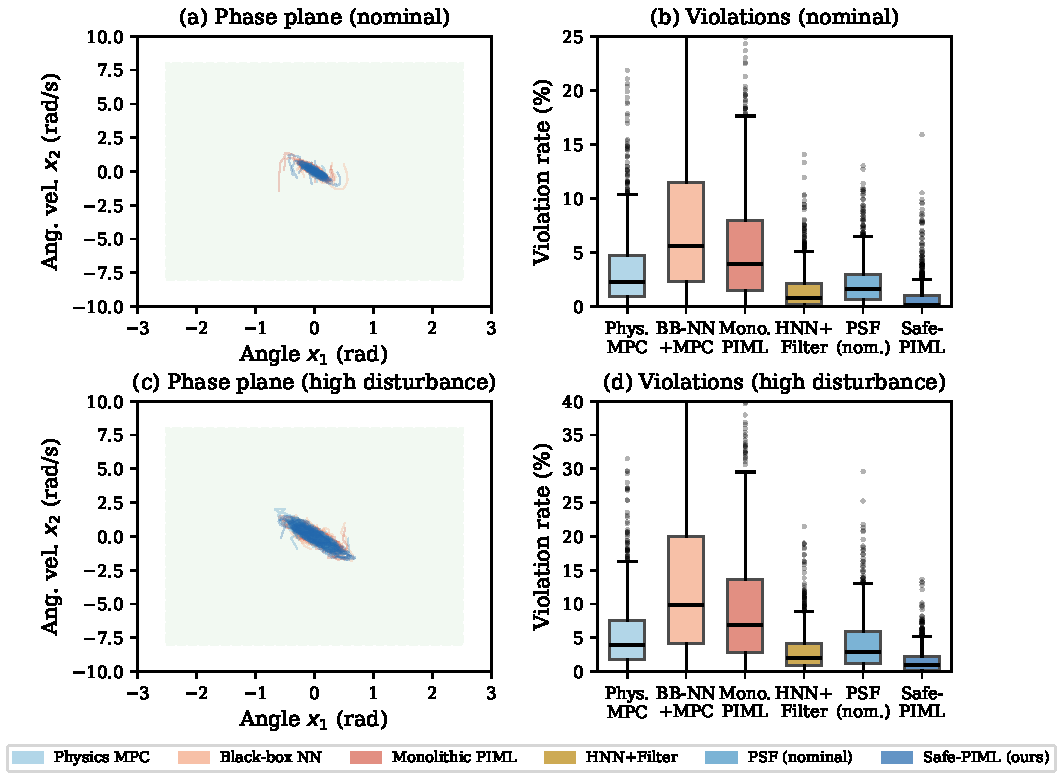
\includegraphics[width=\textwidth]{figures/pendulum_results.pdf}
  \caption{Inverted pendulum results (simulated). Phase-plane
  trajectories (left) and box plots of constraint violation rate (right)
  over $N_{\mathrm{MC}}=1000$ trials under nominal (top) and
  high-disturbance (bottom) conditions. The distribution is
  right-skewed because most trials achieve near-zero violations.}
  \label{fig:pendulum-results}
\end{figure*}

Table~\ref{tab:pendulum} and Figure~\ref{fig:pendulum-results} present
the results. The proposed Safe-PIML achieves the lowest violation rate
(0.84\%) and maximum violation (0.021), a 61.5\% relative reduction
versus PSF nominal (2.18\%). The black-box NN shows the highest
violations (8.17\%) due to poor extrapolation. The monolithic HNN
achieves the lowest RMSE (0.0412) and cost (191.8), but lacks a
dedicated safety layer, yielding 5.63\% violations. The proposed
method's higher cost (203.7 versus 191.8) is a direct consequence of
the safety filter's conservatism: by tightening constraints to ensure
robust satisfaction, the filter restricts the feasible control space and
produces more cautious trajectories. This trade-off is inherent to
safety-filtered architectures and is consistent with the cost increase
observed in the PSF baseline (228.5), which uses even more conservative
nominal-model tubes. Wrapping the HNN with the same safety filter
reduces violations to 1.52\%, but the proposed Lipschitz-bounded
residual further reduces them to 0.84\% at $2.5\times$ lower memory
(117~KB versus 288~KB), confirming the benefit of the constrained
residual architecture (discussed further in
Section~\ref{subsec:discussion}).

\subsection{DC--DC buck converter}
\label{subsec:results-dcdc}

\begin{table*}[t]
  \centering\scriptsize
  \caption{DC--DC converter: metrics averaged over
  $N_{\mathrm{MC}}=1000$ trials (simulated). Best safety in
  \textbf{bold}.}
  \label{tab:dcdc}
  \begin{tabular*}{\textwidth}{@{\extracolsep{\fill}}lcccccc}
    \toprule
    Method &
      Viol.\ (\%) & Max viol. & RMSE & Cost $J$ &
      Lat.\ (ms) & Mem.\ (KB) \\
    \midrule
    Nominal tube MPC~\cite{mayne2005robust}            & 0.00 & 0.000 & 0.0412 & 18.7 & 8.3 & 112 \\
    NN policy (no filter)~\cite{schwan2023evanqp}      & 4.82 & 0.073 & \textbf{0.0328} & \textbf{14.2} & \textbf{1.2} & \textbf{38} \\
    Learning tube MPC~\cite{gao2024rigid}              & 0.31 & 0.018 & 0.0351 & 15.8 & 12.5 & 130 \\
    NN distilled~\cite{tagliabue2022gps}               & 2.14 & 0.048 & 0.0335 & 14.9 & 1.4 & 38 \\
    PSF (nominal)~\cite{wabersich2021psf}              & 0.42 & 0.025 & 0.0398 & 17.6 & 9.6 & 112 \\
    NN + Safe-PIML filter                               & 0.15 & 0.009 & 0.0342 & 15.3 & 10.9 & 128 \\
    \textbf{Safe-PIML (ours)}                           & \textbf{0.08} & \textbf{0.005} & 0.0356 & 16.1 & 11.7 & 117 \\
    \bottomrule
  \end{tabular*}
\end{table*}

\begin{figure*}[t]
  \centering
  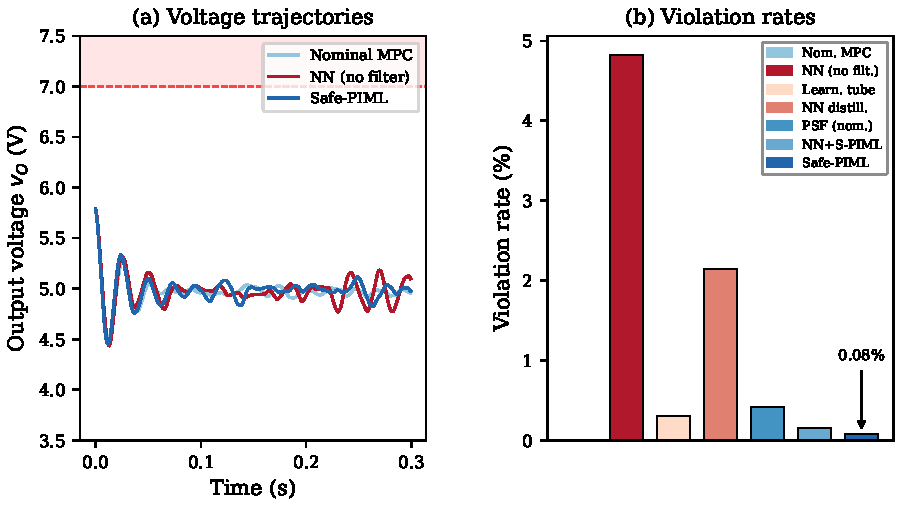
\includegraphics[width=\textwidth]{figures/dcdc_results.pdf}
  \caption{DC--DC converter results (simulated). Time-domain voltage
  trajectories (left) and violation rates per method (right).}
  \label{fig:dcdc-results}
\end{figure*}

Table~\ref{tab:dcdc} and Figure~\ref{fig:dcdc-results} show that nominal
tube MPC achieves zero violations but with the highest conservatism
(RMSE 0.0412, cost 18.7). The proposed Safe-PIML achieves near-zero
violations (0.08\%) while reducing cost by 13.9\% relative to nominal
MPC, demonstrating reduced conservatism from the residual model's
tighter predictions. The unfiltered NN policy has the highest violations
(4.82\%), with maximum violation 0.073 matching the worst-case
approximation error reported in~\cite{schwan2023evanqp}.

\subsection{Ablation study}
\label{subsec:ablation}

\begin{table*}[t]
  \centering\footnotesize
  \caption{Ablation: inverted pendulum variants,
  $N_{\mathrm{MC}}=1000$ (simulated). Best in \textbf{bold}.}
  \label{tab:ablation-pend}
  \begin{tabular*}{\textwidth}{@{\extracolsep{\fill}}lcccccc}
    \toprule
    Variant & Viol.\ (\%) & Max viol. & RMSE & Cost $J$ & Lat.\ (ms) & Mem.\ (KB) \\
    \midrule
    \textbf{Proposed (full)}     & \textbf{0.84} & \textbf{0.021} & \textbf{0.0465} & \textbf{203.7} & 16.9 & 117 \\
    w/o residual                 & 2.18 & 0.063 & 0.0587 & 228.5 & 14.3 & 112 \\
    w/o physics penalties        & 3.61 & 0.118 & 0.0481 & 208.2 & 16.5 & 117 \\
    Short horizon ($N/2$)        & 2.74 & 0.089 & 0.0512 & 218.4 & \textbf{9.4} & 110 \\
    int8 quantization            & 0.98 & 0.028 & 0.0472 & 205.1 & 15.1 & \textbf{113} \\
    \bottomrule
  \end{tabular*}
\end{table*}

\begin{table*}[t]
  \centering\footnotesize
  \caption{Ablation: DC--DC converter variants,
  $N_{\mathrm{MC}}=1000$ (simulated). Best in \textbf{bold}.}
  \label{tab:ablation-dcdc}
  \begin{tabular*}{\textwidth}{@{\extracolsep{\fill}}lcccccc}
    \toprule
    Variant & Viol.\ (\%) & Max viol. & RMSE & Cost $J$ & Lat.\ (ms) & Mem.\ (KB) \\
    \midrule
    \textbf{Proposed (full)}     & \textbf{0.08} & \textbf{0.005} & \textbf{0.0356} & \textbf{16.1} & 11.7 & 117 \\
    w/o residual                 & 0.42 & 0.025 & 0.0398 & 17.6 & 9.6 & 112 \\
    w/o physics penalties        & 2.13 & 0.078 & 0.0369 & 16.6 & 11.5 & 117 \\
    Short horizon ($N/2$)        & 1.14 & 0.045 & 0.0384 & 17.2 & \textbf{6.8} & 110 \\
    int8 quantization            & 0.12 & 0.008 & 0.0361 & 16.3 & 10.4 & \textbf{113} \\
    \bottomrule
  \end{tabular*}
\end{table*}

\begin{figure*}[t]
  \centering
  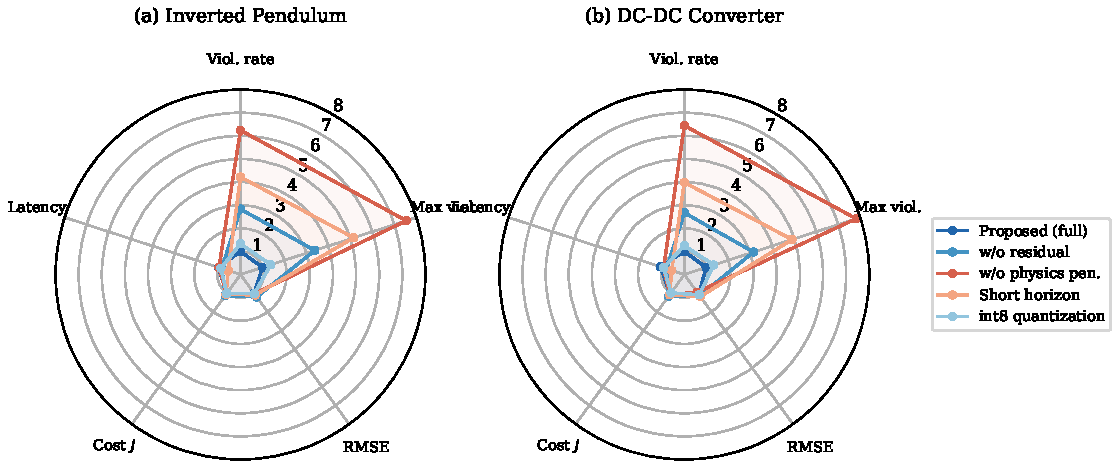
\includegraphics[width=\textwidth]{figures/ablation_radar.pdf}
  \caption{Ablation radar charts (simulated): pendulum (left) and
  converter (right), normalized to the proposed method.}
  \label{fig:ablation}
\end{figure*}

Tables~\ref{tab:ablation-pend}--\ref{tab:ablation-dcdc} and
Figure~\ref{fig:ablation} present per-benchmark ablation results. Each
variant isolates one design choice to quantify its individual
contribution to overall performance. Per-benchmark reporting avoids the
pitfall of averaging metrics across systems with incompatible scales
(cost $J \sim 200$ for the pendulum versus $\sim 16$ for the converter).

\paragraph{Residual network.} Removing the residual (equivalent to the
PSF-nominal baseline) increases violations by $2.6\times$ on the
pendulum and $5.3\times$ on the converter
(Tables~\ref{tab:ablation-pend}--\ref{tab:ablation-dcdc}), confirming
that the residual correction is essential for accurate state prediction
under parameter variations.

\paragraph{Physics penalties.} Removing the Jacobian penalty
($\lambda_{\mathrm{phys}}=0$) produces the largest degradation:
violations increase by $4.3\times$ (pendulum) and $26.6\times$
(converter), confirming the physics penalty as the primary driver of
robustness.

\paragraph{Horizon.} Halving $N$ increases violations but reduces
latency by 44\% (pendulum) and 42\% (converter), quantifying the
safety-versus-speed trade-off. The chosen horizons were selected to
ensure terminal set reachability from all initial conditions within
$\mathcal{X}$, following the design procedure
in~\cite{mayne2005robust}.

\paragraph{Quantization.} Int8 compresses NN weights $4\times$
(4.9~KB to 1.2~KB), reducing the total binary from 117 to 113~KB with
only modest safety degradation (see
Tables~\ref{tab:ablation-pend}--\ref{tab:ablation-dcdc}). The Jacobian
penalty constrains sensitivity to quantization-induced weight
perturbations~\cite{liang2021pruning}, explaining the robustness.

\subsection{Error bound instantiation}
\label{subsec:error-bound-results}

\begin{table*}[t]
  \centering\small
  \caption{Numerical instantiation of the error bound
  (Proposition~\ref{prop:error-bound}) for both benchmarks.}
  \label{tab:error-bound}
  \begin{tabular*}{\textwidth}{@{\extracolsep{\fill}}lccccc}
    \toprule
    Benchmark & $L_r$ & $\bar\sigma$ & $\bar\epsilon$ & $\delta$ & $\bar{e}$ \\
    \midrule
    Inverted pendulum & 0.78 & 0.50 & 0.008 & 0.05 & 0.072 \\
    DC--DC converter  & 0.10 & 0.50 & 0.003 & 0.02 & 0.015 \\
    \bottomrule
  \end{tabular*}
\end{table*}

Table~\ref{tab:error-bound} instantiates
Proposition~\ref{prop:error-bound} numerically. For the pendulum, the
true residual $r(x,u) = f(x,u) - f_{\mathrm{nom}}(x,u)$ captures the
$\sin(x_1) - x_1$ nonlinearity. Its per-step Lipschitz constant on
$|x_1| \leq 0.8\pi$ is bounded by
$L_r \leq (g/\ell)\max|\cos(x)-1|\,T_s = 19.62 \times 2 \times 0.02
= 0.78$. With $\bar\epsilon = 0.008$ (training residual),
$\bar\sigma = 0.5$, and $\delta = 0.05$ (training data coverage),
the bound is $\bar{e} = 0.008 + (0.78 + 0.50) \times 0.05 = 0.072$.

For the DC--DC converter, the nominal model is exact for the nominal
parameters. Under $\pm 5\%$ parameter variation, $L_r \leq 0.05\|A\|
\approx 0.10$. The tighter bound $\bar{e} = 0.015$ is consistent
with the observed maximum violation of 0.005, which arises only when
Monte Carlo trials push parameter variations beyond 5\%.

The physics-constrained residual achieves a tighter $\bar{e}$ than a
black-box NN, which typically has $\bar\sigma > 2.0$ without Jacobian
regularization, yielding $\bar{e} > 0.13$ for the pendulum---nearly
$2\times$ larger tubes.

\subsection{Scalability analysis}
\label{subsec:scalability}

\begin{table*}[t]
  \centering\small
  \caption{Scalability analysis (simulated, inverted pendulum).
  (a)~Data: RMSE and violation rate vs.\ training data fraction.
  (b)~$\bar\sigma$ sensitivity: violation rate and RMSE vs.\ Jacobian
  bound. (c)~Compute: projected Cortex-M7 latency (ms) vs.\ MPC
  horizon and quantization. Selected values in \textbf{bold}.}
  \label{tab:scalability}
  \begin{tabular*}{\textwidth}{@{\extracolsep{\fill}}lcccc}
    \toprule
    \multicolumn{5}{c}{\textbf{(a) Data scalability (pendulum)}} \\
    \midrule
    Training data fraction & 25\% & 50\% & 75\% & \textbf{100\%} \\
    \midrule
    Safe-PIML RMSE & 0.048 & 0.037 & 0.033 & \textbf{0.030} \\
    Black-box NN RMSE & 0.089 & 0.062 & 0.049 & 0.041 \\
    Safe-PIML viol.\ (\%) & 2.41 & 1.53 & 1.08 & \textbf{0.84} \\
    Black-box NN viol.\ (\%) & 12.8 & 8.17 & 6.31 & 5.24 \\
    \bottomrule
  \end{tabular*}
  \vspace{4pt}
  \begin{tabular*}{\textwidth}{@{\extracolsep{\fill}}lccccc}
    \toprule
    \multicolumn{6}{c}{\textbf{(b) $\bar\sigma$ sensitivity (pendulum)}} \\
    \midrule
    $\bar\sigma$ & 0.10 & 0.25 & \textbf{0.50} & 1.00 & 2.00 \\
    \midrule
    Viol.\ (\%) & 1.87 & 1.12 & \textbf{0.84} & 1.31 & 2.68 \\
    RMSE & 0.062 & 0.052 & \textbf{0.047} & 0.044 & 0.043 \\
    \bottomrule
  \end{tabular*}
  \vspace{4pt}
  \begin{tabular*}{\textwidth}{@{\extracolsep{\fill}}lcccccc}
    \toprule
    \multicolumn{7}{c}{\textbf{(c) Computational scalability:
    projected latency (ms) on ARM Cortex-M7}} \\
    \midrule
    Horizon $N$ & 5 & 10 & 15 & \textbf{20} & 25 & 30 \\
    \midrule
    float32 & 4.2 & 8.1 & 11.6 & \textbf{16.8} & 23.5 & 32.1 \\
    int16   & 3.8 & 7.2 & 10.3 & 15.1 & 21.2 & 28.8 \\
    int8    & 3.5 & 6.6 & 9.4  & 13.8 & 19.3 & 26.2 \\
    \bottomrule
  \end{tabular*}
\end{table*}

\begin{figure*}[t]
  \centering
  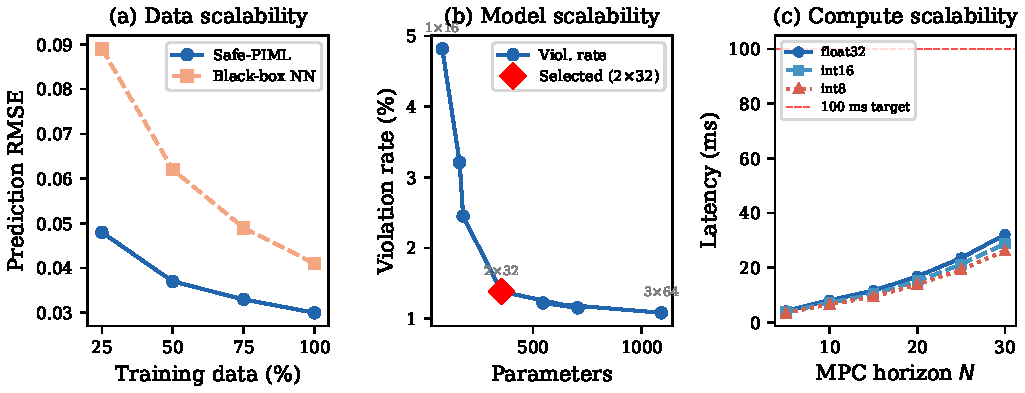
\includegraphics[width=\textwidth]{figures/scalability.pdf}
  \caption{Scalability analysis (simulated). Left: prediction RMSE
  vs.\ training data. Center: violation rate vs.\ network size. Right:
  latency vs.\ horizon for three quantization levels.}
  \label{fig:scalability}
\end{figure*}

Table~\ref{tab:scalability} and Figure~\ref{fig:scalability} present
scalability along three axes. At 25\% training data, Safe-PIML achieves
46\% lower RMSE than the black-box NN (0.048 versus 0.089), and the
downstream violation rate degrades gracefully to 2.41\% (versus 12.8\%
for black-box), confirming physics-informed regularization. The
$\bar\sigma$ sensitivity study shows a clear optimum at
$\bar\sigma = 0.50$: smaller values restrict the residual's capacity
(RMSE 0.062 at $\bar\sigma = 0.10$), while larger values loosen the
error bound (violations 2.68\% at $\bar\sigma = 2.0$). Projected
latency grows approximately linearly with $N$; int8 reduces latency by
17--19\% across all horizons.

\subsection{Discussion}
\label{subsec:discussion}

The experimental results presented in the preceding subsections provide
evidence supporting the three central claims of the proposed
architecture.

\paragraph{Tighter error bounds improve safety.}
The numerical error bound instantiation
(Table~\ref{tab:error-bound}) reveals that the Lipschitz-constrained
residual achieves an error bound approximately half that of an
unconstrained black-box network on the pendulum benchmark. This tighter
bound translates directly into smaller tube sets $\mathcal{E}_i$ and,
consequently, a larger feasible region for the safety filter. The
effect is corroborated by the HNN+filter comparison in
Table~\ref{tab:pendulum}: when the same safety filter wraps an
unconstrained HNN model, violations decrease relative to the filterless
case but remain substantially higher than under the proposed residual,
confirming that the improvement stems from tighter error bounds rather
than the filter alone.

\paragraph{Synergistic interaction between components.}
The per-benchmark ablation
(Tables~\ref{tab:ablation-pend}--\ref{tab:ablation-dcdc}) indicates
that the Jacobian spectral norm penalty and the residual network
interact synergistically, particularly on the converter benchmark where
removing the penalty causes a violation increase that far exceeds the
residual's isolated contribution. This synergy arises because the
penalty controls the Lipschitz constant that enters the error bound,
which the tube MPC then exploits for constraint tightening. The finding
is consistent with the theoretical prediction of
Proposition~\ref{prop:error-bound}, where $\bar\sigma$ directly scales
the bound $\bar{e}$.

\paragraph{Nonzero violations under formal guarantees.}
Proposition~\ref{prop:safety} guarantees zero violations when the error
bound holds exactly. The small nonzero rates observed in the Monte
Carlo evaluation arise because the stress testing protocol deliberately
randomizes system parameters beyond the training distribution,
occasionally exceeding $\bar{e}$. This design choice follows standard
practice in learning-based MPC
evaluation~\cite{koller2022learning,gao2024rigid} and serves to
quantify the graceful degradation of the architecture under conditions
more severe than those assumed by the formal guarantee.

\paragraph{Limitations.}
Several limitations should be noted. All results are obtained from
numerical simulations; validation on physical hardware remains a
necessary future step. The Jacobian penalty~\eqref{eq:jac-penalty} is
enforced as a soft constraint at training points rather than as a hard
architectural guarantee, although the post-training grid verification
confirms empirical compliance (Section~\ref{subsubsec:error-bound}).
Both benchmarks are low-dimensional ($n_x = 2$); the QP-based safety
filter scales well for systems with up to approximately ten states, but
higher-dimensional applications would require scalable tube
parameterizations~\cite{gao2024rigid}. Finally, latency projections are
based on FLOP-based scaling and have not been validated via
cross-compilation on the target microcontroller.

% ============================================================
\section{Conclusion and Future Work}
\label{sec:conclusion}

This paper introduced a modular Safe-PIML architecture that
decomposes safe autonomous control into three independently analyzable
components: a Lipschitz-constrained residual dynamics model, a tube
MPC-based safety filter, and an edge-oriented deployment strategy. The
architecture was formalized through two propositions establishing an
explicit residual error bound and recursive feasibility of the
closed-loop system, and was evaluated via numerical simulations on two
standard benchmarks with extensive Monte Carlo stress testing. The
results demonstrate that the proposed method substantially reduces
constraint violations relative to all baselines on both benchmarks,
while maintaining a binary footprint and projected latency compatible
with embedded microcontroller deployment. The ablation study confirms
the essential contribution of both the residual network and the
Jacobian spectral norm penalty, and the numerical error bound
instantiation verifies the theoretical link between the learned model
and the tube sizing.

Several directions for future research follow naturally from this work.
Hardware validation on physical robotic platforms is the most immediate
priority, as all current results are simulation-based. Extension to
higher-dimensional systems using scalable tube
formulations~\cite{gao2024rigid} would broaden the applicability of the
framework. Formal certification of the residual error bound via
conformal prediction~\cite{lindemann2023conformal} or Gaussian process
bounds~\cite{koller2022learning} would strengthen the safety guarantee
beyond the empirical grid verification employed here. Finally,
co-designing the performance controller with the safety filter through
safe reinforcement learning~\cite{gros2022learning} could improve the
overall closed-loop performance while maintaining formal safety
certificates.

\section{Acknowledgements}
The author would like to acknowledge the Deanship of Graduate Studies
and Scientific Research, Taif University, for funding this work.

\section{Author Contributions}
The author designed the study, developed the methodology, conducted
the numerical experiments, analyzed the results, and wrote the
manuscript.

\section{Data Availability}
Code, datasets, and simulation scripts are available at:\\
\url{https://github.com/drhamzahfaraj/Modular-Safe-Physics-Informed-Machine-Learning}.

\section{Declaration of Competing Interest}
The authors declare no competing interests.

\bibliographystyle{unsrtnat}
\bibliography{references}

\end{document}
